\documentclass[11pt,a4paper]{article}

\usepackage[T1]{fontenc}
\usepackage[utf8]{inputenc}
\usepackage[margin=0.85in]{geometry}
\usepackage{amsmath,amssymb,bm}
\usepackage{booktabs}
\usepackage{array}
\usepackage{graphicx}
\usepackage{caption}
\usepackage{xcolor}
\usepackage{hyperref}
\usepackage{tikz}
\usetikzlibrary{arrows.meta,positioning,fit}

\hypersetup{
  colorlinks=true,
  linkcolor=blue!55!black,
  urlcolor=blue!55!black,
  citecolor=blue!55!black
}

\graphicspath{{./}{report_figures/}}

\newcommand{\state}{\bm{x}}
\newcommand{\meas}{\bm{z}}
\newcommand{\prior}{\state_k^-}
\newcommand{\post}{\state_k^+}
\newcommand{\gain}{K}
\newcommand{\trust}{\bm{\gamma}}
\newcommand{\avail}{\bm{a}}
\newcommand{\innov}{\bm{r}}
\newcommand{\wrap}{\operatorname{wrap}}
\newcommand{\diag}{\operatorname{diag}}

\title{\vspace{-1em}Robust Gamma-KalmaNet State Estimation for QCar under Sensor Faults}
\author{Quang Huy Nugyen \and Echrak Chnib}

\date{\today}

\begin{document}
\maketitle

\begin{abstract}
This article presents a robust KalmaNet-style state estimator for the QCar
platform. The estimator preserves a physics-based vehicle prediction model and
learns the uncertain part of the filtering problem: how much each measurement
should be trusted and how strongly the state should be corrected. The learned
measurement trust vector is denoted by $\trust_k$ and acts as a ``robust
gamma'' gate. The proposed estimator tracks $\state=[x,y,\psi,v]^T$ using GPS
position, fused heading, tachometer velocity, IMU, steering, and wheel-speed
information. Training combines real QCar driving data with synthetic GPS,
heading, velocity, IMU, steering, and wheel-speed faults. The learned estimator
reduces attacked validation loss from 1.1095 to 0.4028 and improves four-state
RMSE compared with a kinematic reference in offline validation. The result is a
hybrid observer: vehicle physics provides the prior state, while a recurrent
neural update learns when corrupted measurements should be down-weighted.
\end{abstract}

\section{Introduction}

Autonomous QCar experiments require a state estimate that is accurate enough
for feedback control and stable enough during bad sensor periods. A standard
Extended Kalman Filter (EKF) is a strong baseline when its assumptions are
correct. It uses a vehicle model for prediction and a measurement model for
correction. However, the EKF can become fragile when the measurement noise is
not just random noise but a structured fault: GPS jumps, GPS dropout, frozen
velocity, wheel speed scaling, heading glitches, or short IMU bursts. In those
cases the filter may apply a correction in the wrong direction because the
measurement is still treated as believable.

This work develops a robust KalmaNet-style estimator for the QCar.
The key design choice is simple:
\begin{quote}
  keep the vehicle model for prediction, and learn a trust-controlled update
  for difficult sensor behavior.
\end{quote}
The learned trust vector $\trust_k$ is the important element. When a channel is
clean, its trust should stay high. When a channel is attacked or unavailable,
its trust should decrease so that the innovation cannot force a large state
jump. This is close in spirit to KalmanNet \cite{revach2022kalmannet} and
RobustStateNet \cite{dahal2024robuststatenet}, but the proposed QCar estimator
is more conservative: the prediction step is an analytical bicycle model rather
than a learned predictor.

\section{Problem Definition}

\subsection{State and Measurement}

The estimated state is
\begin{equation}
  \state_k =
  \begin{bmatrix}
    x_k & y_k & \psi_k & v_k
  \end{bmatrix}^{T},
\end{equation}
where $x$ and $y$ are global position, $\psi$ is heading, and $v$ is forward
velocity. Yaw rate is recorded as an auxiliary signal in some experiments, but
the estimator evaluated in this article uses the four-state representation
above.

The measurement vector is
\begin{equation}
  \meas_k =
  \begin{bmatrix}
    x_{gps,k} & y_{gps,k} & \psi_{fused,k} & v_{tach,k}
  \end{bmatrix}^{T},
  \qquad
  \meas_k = H\state_k + \bm{n}_k,
  \qquad
  H \approx I_4 .
\end{equation}
The measured heading is reconstructed using the same heading-fusion procedure
as the onboard estimator. GPS availability metadata is retained because it is
essential for distinguishing sensor faults from normal innovation.

\subsection{Raw Sensor Inputs}

The model receives raw inputs grouped by physical source:
\begin{itemize}
  \item IMU branch: velocity context, heading context, acceleration, and yaw
  rate;
  \item steering branch: velocity context, heading context, and steering angle;
  \item wheel branch: velocity context, heading context, and four wheel-speed
  channels;
  \item availability metadata: GPS valid flag, heading valid flag, GPS hold
  flag, and GPS age.
\end{itemize}

This separation matters because each sensor family has different failure
behavior. GPS position can jump or disappear. Velocity can freeze or become
scaled. IMU signals can become noisy or biased. The learned update uses these
signals to decide whether the current measurement should be trusted.

\section{Estimator Architecture}

Figure~\ref{fig:architecture} shows the estimator at a high level. The
prediction side is deterministic. The update side is learned and recurrent.

\begin{figure}[htbp]
\centering
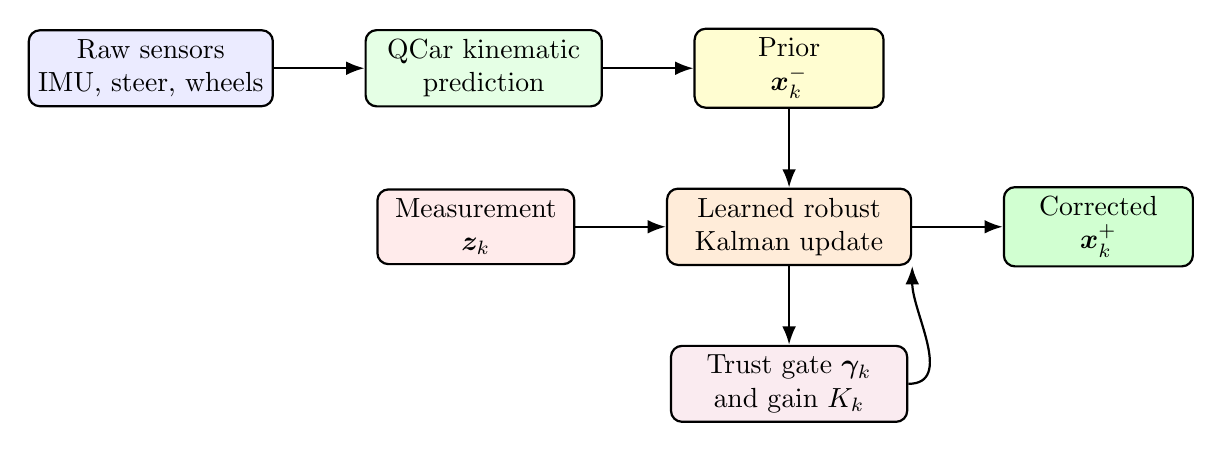
\begin{tikzpicture}[node distance=1.0cm and 1.15cm,>=Latex,thick]
  \node[draw,rounded corners,align=center,fill=blue!8,
        minimum width=2.8cm,minimum height=0.9cm] (raw)
        {Raw sensors\\IMU, steer, wheels};
  \node[draw,rounded corners,right=of raw,align=center,fill=green!10,
        minimum width=3.0cm,minimum height=0.9cm] (pred)
        {QCar kinematic\\prediction};
  \node[draw,rounded corners,right=of pred,align=center,fill=yellow!18,
        minimum width=2.4cm,minimum height=0.9cm] (xp)
        {Prior\\$\prior$};
  \node[draw,rounded corners,below=1.0cm of xp,align=center,fill=orange!15,
        minimum width=3.1cm,minimum height=0.9cm] (upd)
        {Learned robust\\Kalman update};
  \node[draw,rounded corners,left=of upd,align=center,fill=red!8,
        minimum width=2.5cm,minimum height=0.9cm] (z)
        {Measurement\\$\meas_k$};
  \node[draw,rounded corners,right=of upd,align=center,fill=green!18,
        minimum width=2.4cm,minimum height=0.9cm] (xu)
        {Corrected\\$\post$};
  \node[draw,rounded corners,below=of upd,align=center,fill=purple!8,
        minimum width=3.0cm,minimum height=0.8cm] (trust)
        {Trust gate $\trust_k$\\and gain $K_k$};

  \draw[->] (raw) -- (pred);
  \draw[->] (pred) -- (xp);
  \draw[->] (xp) -- (upd);
  \draw[->] (z) -- (upd);
  \draw[->] (upd) -- (xu);
  \draw[->] (upd) -- (trust);
  \draw[->] (trust.east) to[out=0,in=-90] (upd.south east);
\end{tikzpicture}
\caption{Hybrid RKNet structure used in this work. The prior is generated by
QCar physics. The neural update learns a measurement trust gate and a
Kalman-style gain.}
\label{fig:architecture}
\end{figure}

\subsection{Kinematic Prediction}

The prediction step has no learned parameters. It is a bicycle-model update
with wheelbase $L$:
\begin{equation}
  \dot{\psi}_k =
  \frac{v_k\tan(\delta_k)}{L},
\end{equation}
where $\delta_k$ is the steering angle. The predicted pose is
\begin{align}
  x_k^- &= x_{k-1}^+ + v_{pose,k}\cos(\psi_{k-1}^+)\Delta t, \\
  y_k^- &= y_{k-1}^+ + v_{pose,k}\sin(\psi_{k-1}^+)\Delta t, \\
  \psi_k^- &=
  \wrap\left(\psi_{k-1}^+
  + \frac{v_{pose,k}\tan(\delta_k)}{L}\Delta t\right).
\end{align}

Longitudinal velocity is predicted with a first-order lag model from the
previous velocity and throttle:
\begin{equation}
  \dot{v}_k =
  \frac{-v_{k-1}^+ + g u_k}{\tau},
  \qquad
  v_k^- =
  \operatorname{clip}\left(v_{k-1}^+ + \dot{v}_k\Delta t\right).
\end{equation}
The numerical parameters used in the experiments are $L=0.2$, $\tau=0.301$,
$g=6.598$, $|v|\leq2.0$ m/s, and maximum acceleration $2.0$ m/s$^2$.

\subsection{Learned Robust Update}

The learned update receives the prior $\prior$, the previous corrected state
$\state_{k-1}^+$, the current measurement $\meas_k$, the previous measurement
$\meas_{k-1}$, and availability metadata. It forms three main residual terms:
\begin{align}
  \Delta \state_k &= \wrap(\state_k^- - \state_{k-1}^{+}), \\
  \innov_k &= \wrap(\meas_k - H\state_k^-), \\
  \Delta \meas_k &= \wrap(\meas_k - \meas_{k-1}).
\end{align}

The hard availability vector is
\begin{equation}
  \avail_k =
  \begin{bmatrix}
    g_k & g_k & h_k & 1
  \end{bmatrix}^{T},
\end{equation}
where $g_k$ is the GPS-position valid flag and $h_k$ is the heading valid flag.
Unavailable measurement channels are removed before the learned correction.

The update feature vector is
\begin{equation}
\begin{aligned}
  \bm{f}_k =
  [&\Delta\state_k / \bm{s}_x,\,
    (\avail_k \odot \innov_k) / \bm{s}_z,\,
    (\avail_k \odot \Delta\meas_k) / \bm{s}_z,\,
    \avail_k,\\
   &g^{hold}_k,\,
    \log(1+\min(age_k,10)),\,
    \log(1+|\avail_k\odot\innov_k|),\,
    \log(1+|\avail_k\odot\Delta\meas_k|)] .
\end{aligned}
\end{equation}
For the four-state model this gives a 26-dimensional update feature vector.
The scale vectors used for normalization are
\[
  \bm{s}_x=\bm{s}_z=[0.25,\ 0.25,\ 0.20,\ 0.50].
\]

The robust gamma/trust vector is generated by a small MLP:
\begin{equation}
  \trust_k = \sigma(MLP_{\gamma}(\bm{f}_k)).
\end{equation}
Only the measurement part of this vector is used directly as the measurement
trust gate. Clean channels should stay close to one; attacked channels should
move toward zero.

The Kalman-style gain is generated by a GRU and an MLP:
\begin{align}
  \bm{h}_k &= GRU(\trust_k \odot \bm{f}_k,\bm{h}_{k-1}), \\
  K_k &= s\tanh(MLP_K(\bm{h}_k)).
\end{align}
The gain output is bounded with $s=1.2$. Exponential smoothing is also applied
to the gain and trust gate with $\alpha=0.35$.

The corrected state is
\begin{equation}
  \state_k^+
  =
  \state_k^-
  +
  K_k
  \left(
    \avail_k \odot \trust_k^z \odot \innov_k
  \right),
  \label{eq:robust_update}
\end{equation}
where $\trust_k^z$ is the measurement-trust part of the learned gate. Equation
\eqref{eq:robust_update} is the main robustness mechanism. A corrupted GPS or
velocity measurement may create a large innovation, but the innovation is first
multiplied by the learned trust gate before it reaches the gain. The runtime
also clamps the per-step correction to
\[
  [0.35,\ 0.35,\ 0.35,\ 0.80]
\]
for $[x,y,\psi,v]$.

\section{Dataset and Training}

\subsection{Experimental Data}

The experimental data consists of time-aligned QCar sensor signals, measurement
vectors, reference state estimates, timestamps, and sensor availability
metadata. The main training sequence contains 52,921 samples over 671.84
seconds of driving, with a mean timestep of 0.0127 seconds. The supervised
target is a clean EKF reference estimate rather than motion-capture ground
truth.

\begin{table}[htbp]
\centering
\caption{Main experimental data and training settings.}
\label{tab:dataset}
\begin{tabular}{ll}
\toprule
Item & Value \\
\midrule
State order & $[x,y,\psi,v]$ \\
Measurement order & $[x_{gps},y_{gps},\psi_{fused},v_{tach}]$ \\
Training sequence & Real QCar driving data \\
Samples / duration & 52,921 samples / 671.84 s \\
Mean timestep & 0.0127 s \\
Validation split & final 20\% of sequence \\
Training windows & $T=50$ for Phase B, $T=80$ for Phase C \\
Predictor mode & kinematic QCar bicycle model \\
Updater hidden size & 32 \\
Gain hidden size & 32 \\
Optimizer learning rate & $1.0\times10^{-4}$ \\
\bottomrule
\end{tabular}
\end{table}

\subsection{Training Phases}

Because the predictor used in this study is kinematic, predictor pretraining is
not required. The useful training phases are:
\begin{itemize}
  \item Phase B: freeze the predictor and train only the learned updater;
  \item Phase C: fine tune the complete recurrent runtime loop with teacher
  forcing disabled.
\end{itemize}

The state loss is weighted MSE:
\begin{equation}
  L_{state}
  =
  \frac{1}{N}\sum_k
  \left\|
  W^{1/2}(\hat{\state}_k-\state_k^\star)
  \right\|_2^2,
  \qquad
  W=[1.0,\ 1.0,\ 2.5,\ 1.2].
\end{equation}

The full loss combines state accuracy, trust supervision, gain regularization,
and temporal smoothness:
\begin{equation}
\begin{aligned}
  \mathcal{L}
  &=
  \lambda_u L_{upd}
  + \lambda_p L_{pred}
  + \lambda_{\gamma} L_{\gamma}
  + \lambda_K L_K
  + \lambda_{\Delta K} L_{\Delta K}
  + \lambda_{\Delta\gamma} L_{\Delta\gamma}.
\end{aligned}
\end{equation}
The Phase C weights are $\lambda_u=0.85$ and $\lambda_p=0.15$.
Measurement-mask supervision uses a clean target of one and an attacked target
of zero for each affected measurement channel.

\section{Sensor Attack Augmentation}

The training data is not only clean driving. Synthetic attacks are injected
offline so the model sees examples of sensor faults and receives supervision
for which channels should be trusted.

\begin{table}[htbp]
\centering
\caption{Sensor-fault augmentation configuration used in the experiments.}
\label{tab:augmentation}
\begin{tabular}{lll}
\toprule
Attack group & Probability & Enabled failure types \\
\midrule
Raw branch attack & 0.25 & bias, scale, freeze, noise, ramp, zero-out \\
Direct measurement attack & 0.35 & heading and velocity corruption \\
GPS position attack & 0.45 & noise, freeze, jump, dropout, reacquisition \\
Maximum raw branches attacked & 1 & one of IMU, steering, wheel \\
\bottomrule
\end{tabular}
\end{table}

The GPS attacks are especially important for QCar because GPS position directly
drives $x$ and $y$ correction. A jump attack can make the EKF snap to a wrong
position unless the measurement is down-weighted. A dropout attack is different:
the availability gate should remove $x/y$, while the learned update continues
using the remaining channels.

\section{Results}

\subsection{Training History}

The training history contains 20 logged epochs after predictor pretraining was
omitted. The model selected for robustness corresponds to epoch 15 in Phase B.
Table~\ref{tab:train_result} summarizes the main points.

\begin{table}[htbp]
\centering
\caption{Training history. Selection loss combines clean and attacked
validation, with attacked validation weighted more strongly.}
\label{tab:train_result}
\begin{tabular}{lcccc}
\toprule
Model point & Epoch & Clean val. & Attacked val. & Selection loss \\
\midrule
First logged epoch & 1 & 0.00668 & 1.10951 & 0.66838 \\
Selected robust model & 15 & 0.01751 & 0.40279 & 0.24868 \\
Final Phase C model & 20 & 0.02408 & 0.43457 & 0.27037 \\
\bottomrule
\end{tabular}
\end{table}

The attacked validation loss decreases from 1.10951 to 0.40279 at the selected
robust model, a reduction of about 63.7\%. The clean validation loss is higher
at the robust model than at the first clean-only epoch. This is an expected
tradeoff: the estimator becomes more conservative so it can survive corrupted
measurements.

\subsection{Offline Validation}

Offline validation compares a kinematic reference and the learned RKNet model
against the EKF target on an independent driving sequence. Some recorded
signals contain an auxiliary yaw-rate channel, so Table~\ref{tab:offline_rmse}
reports only the four-state surface used by the proposed estimator.

\begin{table}[htbp]
\centering
\caption{Offline RMSE against the EKF target on an independent validation
sequence.}
\label{tab:offline_rmse}
\begin{tabular}{lccccc}
\toprule
Method & $x$ [m] & $y$ [m] & $\psi$ [rad] & $v$ [m/s] & Mean, four states \\
\midrule
Kinematic reference & 0.0663 & 0.0574 & 0.1151 & 0.0134 & 0.0631 \\
Learned RKNet & 0.0076 & 0.0168 & 0.1096 & 0.0124 & 0.0366 \\
\bottomrule
\end{tabular}
\end{table}

The learned estimator strongly improves $x$ and $y$ RMSE and gives a smaller
four-state mean RMSE. Heading remains the hardest channel. This is reasonable
because heading is affected by angle wrapping, GPS heading availability, and
the reference itself.

\subsection{Runtime Comparator Run}

A representative runtime comparison contains 8,413 model samples over 95.97
seconds, with no fallback samples. It includes five attack segments and 1,510
attack-active samples. Only 421 samples had fresh GPS, while 8,380 used GPS
hold validity, so this run is useful for checking robustness during limited
fresh GPS availability.

\begin{figure}[htbp]
\centering
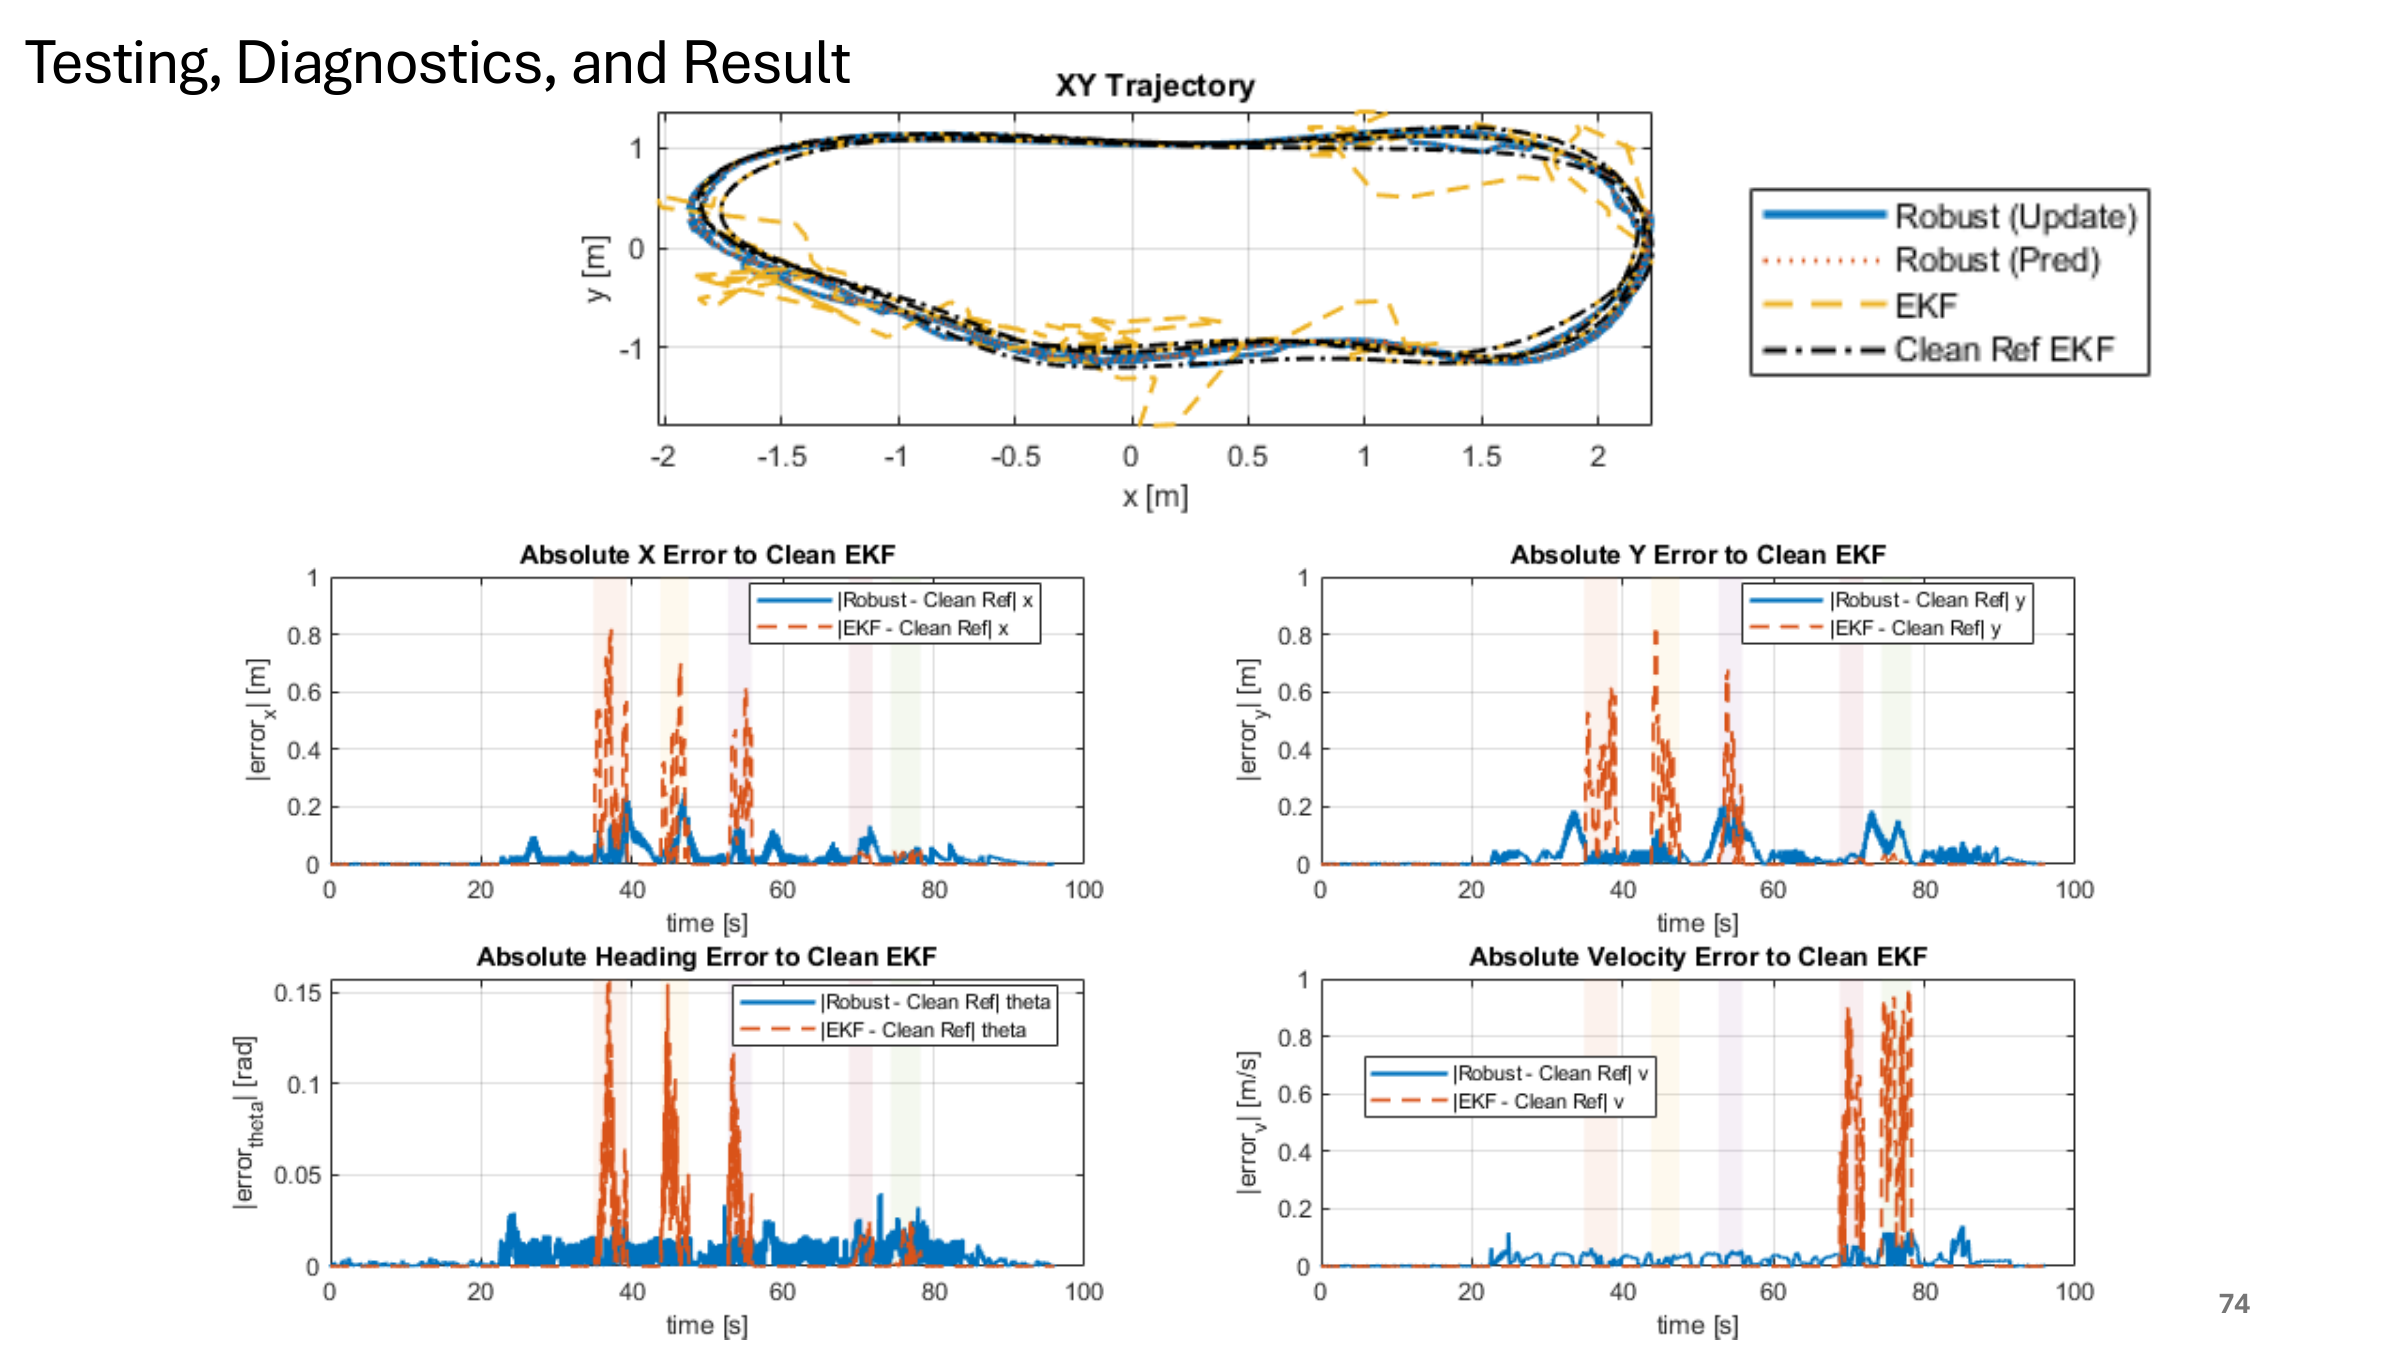
\includegraphics[width=0.98\linewidth]{kalmarobust_result-12.png}
\caption{State-estimation behavior during the runtime comparison. The robust
estimator follows the clean-reference EKF while the ordinary EKF shows larger
spikes during attack intervals.}
\label{fig:pdf_result_state}
\end{figure}

\clearpage

\begin{figure}[htbp]
\centering
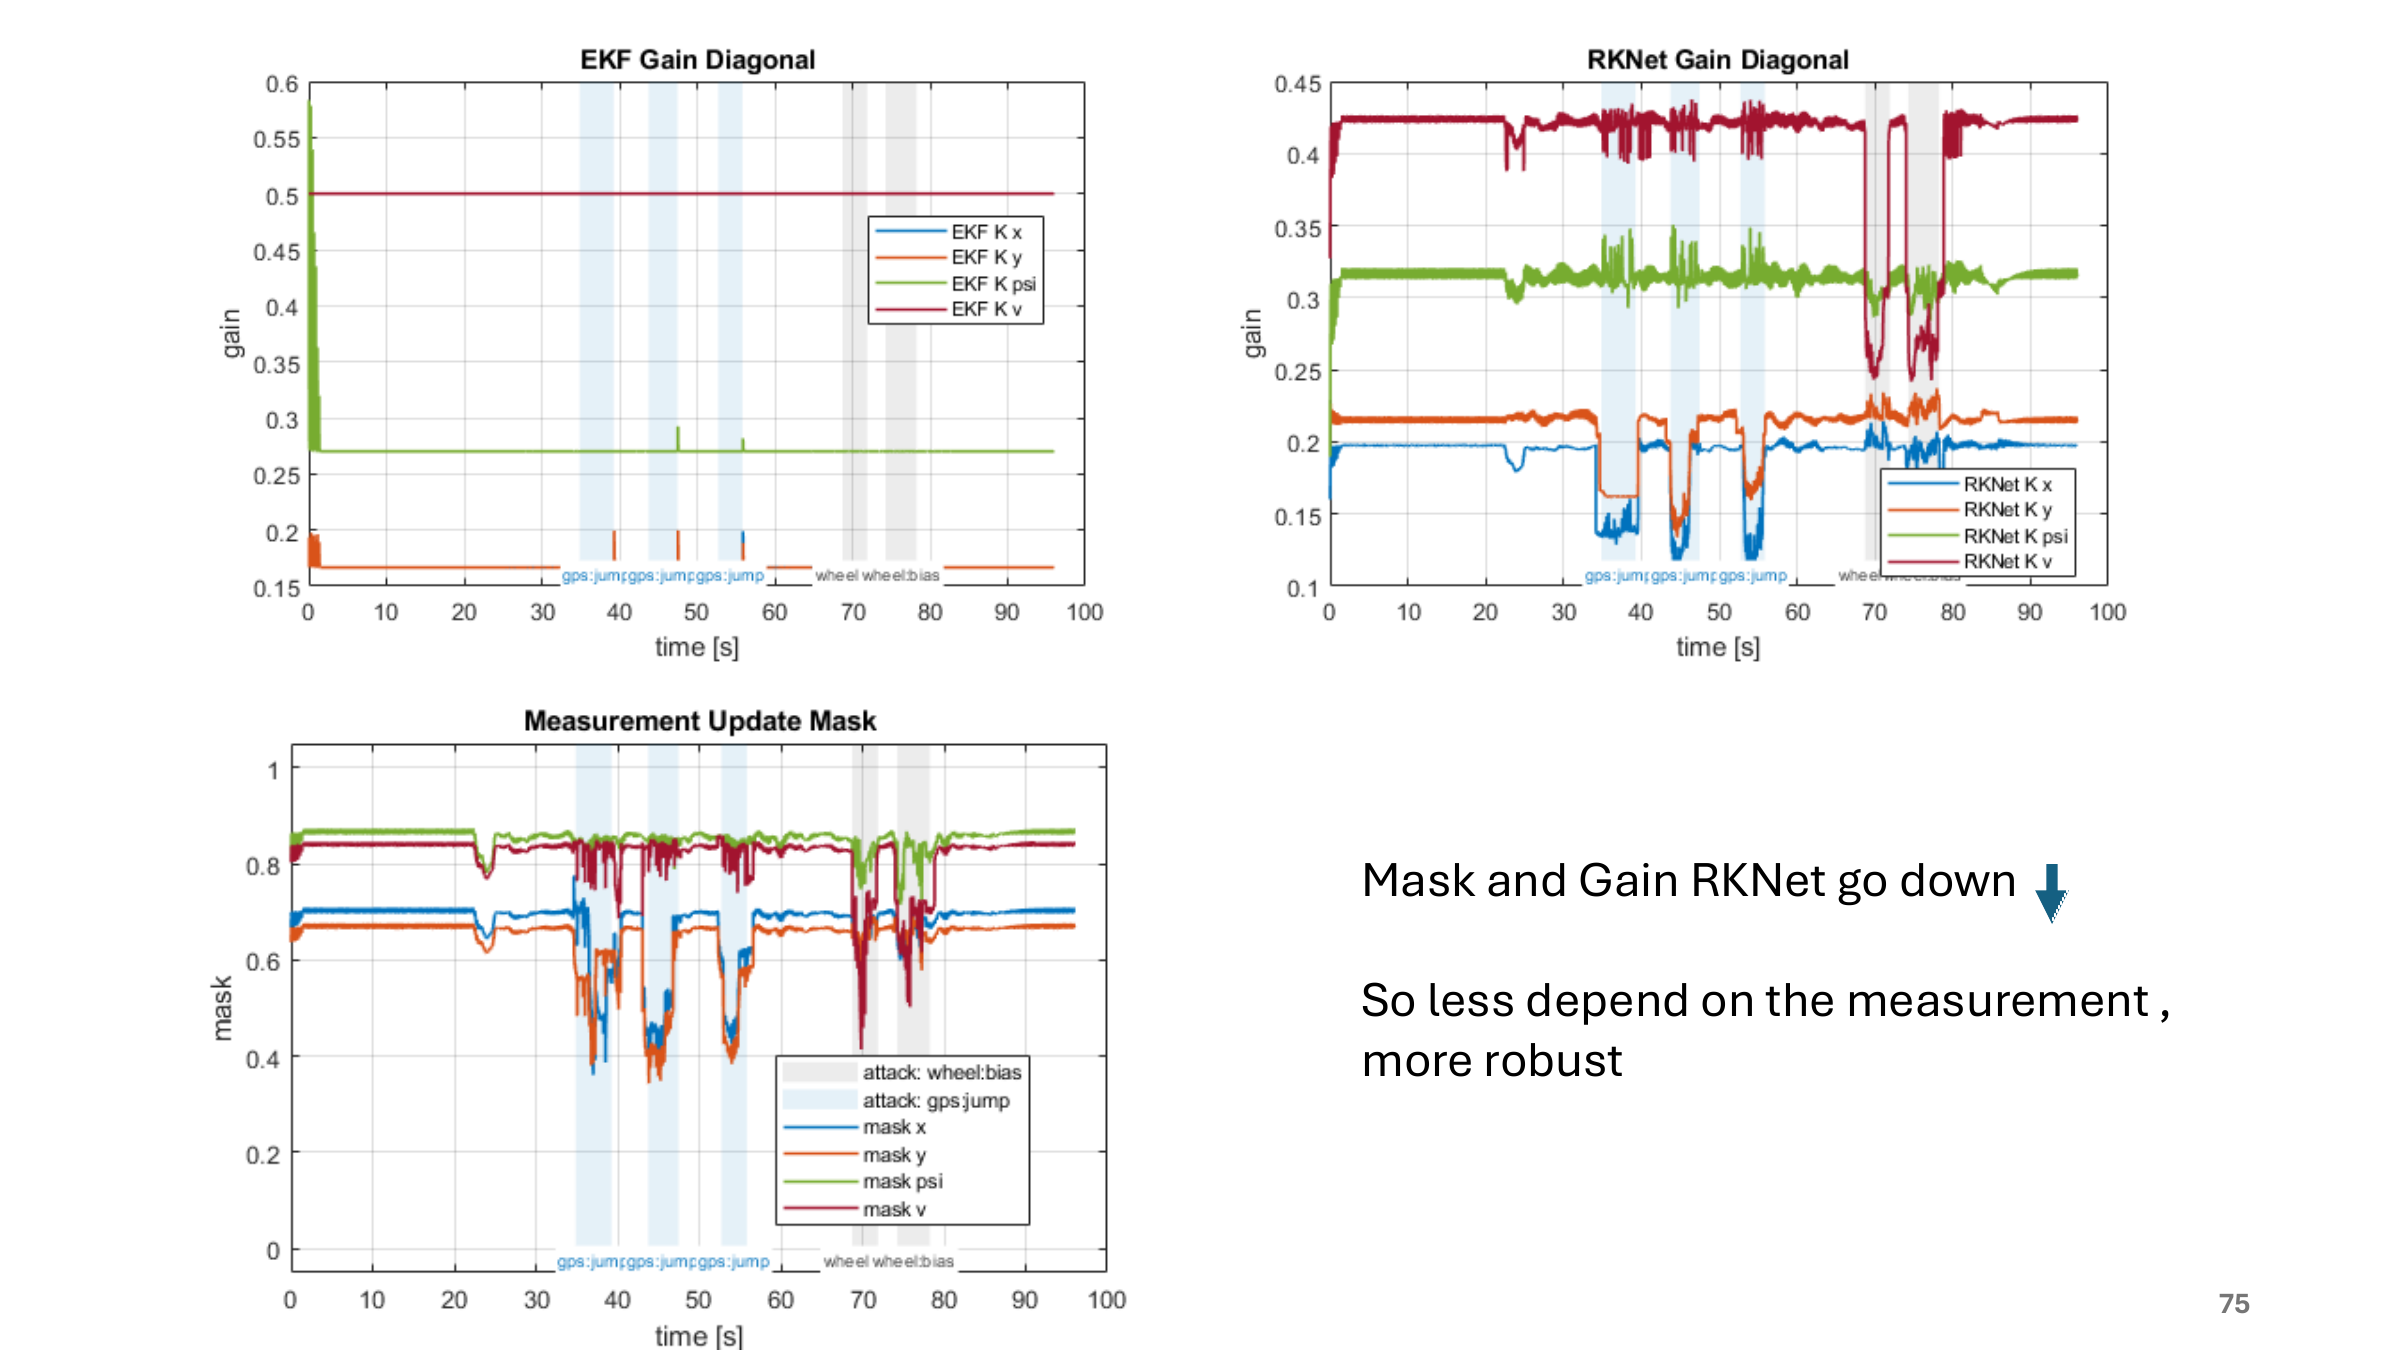
\includegraphics[width=0.98\linewidth]{kalmarobust_result-13.png}
\caption{Gain and measurement-mask behavior during the runtime comparison. The
learned mask and effective gain decrease during GPS jump and wheel-bias
intervals, reducing dependence on corrupted measurements.}
\label{fig:pdf_result_mask}
\end{figure}

Figures~\ref{fig:pdf_result_state} and~\ref{fig:pdf_result_mask} show the main
behavior expected from the robust gamma gate. During the GPS jump intervals,
the measurement mask for position decreases and the effective diagonal gain
also drops. During wheel-bias intervals, the velocity-side trust and gain become
more conservative. This means the update is not blindly following the
measurement; it is using the innovation only after passing it through the
learned reliability gate.

\section{Discussion}

The important engineering result is the separation of responsibilities.
The QCar prediction step carries the vehicle kinematics and basic longitudinal
behavior. The neural update does not need to relearn the full vehicle model.
Instead, it learns the part that is hard to tune manually: the measurement
trust policy under abnormal sensor conditions.

The learned trust mechanism also makes the estimator more interpretable than a
single end-to-end recurrent network. The plotted $\trust_k$ values show when
the estimator is reducing confidence in GPS position, heading, or velocity.
The gain plots show whether the final correction is aggressive or conservative.
This is useful for debugging because a bad output can be traced to three
quantities: the prior state, the innovation, and the trust/gain pair.

There are also limitations:
\begin{itemize}
  \item the target is an EKF/reference estimator, not absolute ground truth;
  \item the attacks are synthetic, so real hardware failures still need more
  dedicated experiments;
  \item the present predictor is kinematic, so raw-branch learned feature
  masking is not used in the prediction path;
  \item the model is trained mainly on the available QCar driving sequences and
  should be rechecked before claiming generalization to other vehicles or
  tracks;
  \item the clean/robust tradeoff is visible: robustness improves attacked
  validation loss, while clean validation loss becomes slightly worse.
\end{itemize}

\section{Conclusion}

The robust gamma-KalmaNet estimator developed in this work is a practical
hybrid state estimator for QCar. It preserves a deterministic QCar kinematic
prediction model and learns a recurrent Kalman-style update with a measurement
trust gate. The trust gate suppresses corrupted GPS, heading, and velocity
channels before the innovation is applied to the state. Training with synthetic
sensor attacks reduces attacked validation loss substantially, and offline
validation shows lower four-state RMSE than the kinematic reference on an
independent validation sequence. The result is an estimator that is still close
to the filtering structure used in classical observers, but with a learned
robustness layer where hand-tuned noise models are weakest.

\section*{Data and Code Availability}

The implementation and experimental material are maintained in the project
repository. The results in this article are based on real QCar driving
sequences with synthetic sensor-fault augmentation. The reported metrics can be
reproduced by training the robust update on the described data split and
evaluating the selected model on an independent validation sequence.

\begin{thebibliography}{9}

\bibitem{revach2022kalmannet}
G. Revach, N. Shlezinger, X. Ni, A. L. Escoriza, R. J. G. van Sloun, and
Y. C. Eldar, ``KalmanNet: Neural network aided Kalman filtering for partially
known dynamics,'' \emph{IEEE Transactions on Signal Processing}, vol. 70,
pp. 1532--1547, 2022.

\bibitem{dahal2024robuststatenet}
P. Dahal, S. Mentasti, L. Paparusso, S. Arrigoni, and F. Braghin,
``RobustStateNet: Robust ego vehicle state estimation for Autonomous Driving,''
\emph{Robotics and Autonomous Systems}, vol. 172, article 104585, 2024.

\end{thebibliography}

\end{document}
